\chapter{Disciplina}
\index{Disciplina}

Neste capítulo serão apresentadas informações importantes para a melhor compreensão e organização da disciplina.

\section{Participante}
\index{Participante}

Ao clicar em \textbf{Participantes}, no bloco \textbf{Participantes da disciplina}, abre-se uma página com a lista de pessoas que estão vinculadas a esta disciplina. Essa lista permite muitos filtros, que tem por objetivo auxiliar o usuário a buscar um aluno, professor ou tutor. 
A Tabela \ref{table:filtrosParticipantes} contém mais detalhes das opções de flitros disponíveis.

\begin{table}[htbp]
\begin{flushleft}
%\begin{wraptable}{t}[5pt]{6cm}
\begin{tabular}{p{6cm}|p{8cm}} \hline
\vspace{0.1cm} 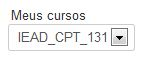
\includegraphics[width=2.2cm]{imagem/cap3/fig1.jpg} & No menu \textbf{Meus cursos} pode-se mudar para a lista de Participantes de outras disciplinas da qual se faça parte.\\ %\hline
\vspace{0.1cm} 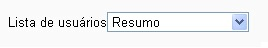
\includegraphics[width=4cm]{imagem/cap3/fig4.jpg}&Em \textbf{Lista de usuários} se escolhe entre uma lista resumida, ou outra mais completa, com mais dados de cada participante.\\%\hline
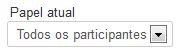
\includegraphics[width=3cm]{imagem/cap3/fig5.jpg}&Papel atual filtra pela função que o participante exerce na disciplina, se é professor, tutor, aluno, etc.\\\hline
\end{tabular}
\caption{Filtros de Participantes}
  \label{table:filtrosParticipantes}
\end{flushleft}
\end{table}%

É possível ordenar uma lista usando o seu cabeçalho como illustra a Figura \ref{fig:cabecalhoLista}.

\begin{figure}[htbp]
 \begin{center}
 \fbox{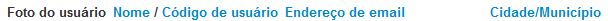
\includegraphics[width=0.7\textwidth]{imagem/cap3/fig6.jpg}}
  \caption{Cabeçalho de Listas}
  \label{fig:cabecalhoLista}
 \end{center}
\end{figure}

Ao clicar em um dos cabeçalhos, por exemplo, em \textbf{Nome}, ordena-se a lista segundo o nomes dos participantes. Clicando uma vez, a lista é ordenado em ordem crescente, e clicando mais uma vez, em ordem decrescente.

No topo da lista é possível ver dois menus alfabéticos como na Figura \ref{fig:filtroNomes}. Clicando numa das letras filtra a lista pela letra escolhida, seja \textbf{Nome}, ou \textbf{Sobrenome}. Associando isso ao ordenamento da lista por \textbf{Nome}, por exemplo, tem-se uma ferramenta de grande utilidade.

\begin{figure}[htbp]
 \begin{center}
 \fbox{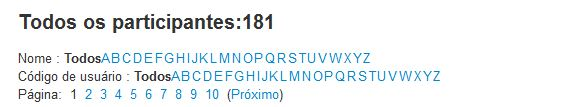
\includegraphics[width=0.4\textwidth]{imagem/cap3/fig7.jpg}}
  \caption{Filtro de Nomes}
  \label{fig:filtroNomes}
 \end{center}
\end{figure}

Sem esquecer que, ao clicar-se em cada nome da lista abrirá o perfil público deste.

Outra funcionalidade da \textbf{lista de Participantes} é a que permite enviar mensagens coletivas através da plataforma:
Primeiro filtra-se a lista até obter o grupo com o qual se deseja enviar mensagens. Por exemplo: alunos que não acessam a disciplina há mais de cinco dias.
No inferior da página, clica-se em \textbf{Mostrar todos os \#\#} (onde \#\# é o número de listados após configurar os filtros).
Clica-se então no botão \textbf{Selecionar Tudo}. No menu \textbf{Com os usuários selecionados} escolher \textbf{Enviar uma mensagem} (Veja a Figura \ref{fig:enviarMensagem}).

\begin{figure}[htbp]
 \begin{center}
 \fbox{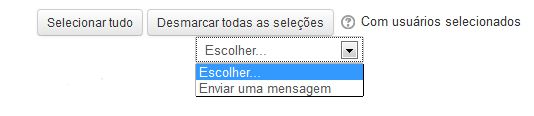
\includegraphics[width=0.5\textwidth]{imagem/cap3/fig8.jpg}}
  \caption{Enviar mensagem}
  \label{fig:enviarMensagem}
 \end{center}
\end{figure}
Abrirá uma página com um editor de texto semelhante ao já encontrado em outras partes do Moodle, onde se pode escrever a mensagem. Abaixo desta estará uma lista com os destinatários escolhidos, onde ainda será possível \textbf{Remover} algum que tenha sido colocado inadvertidamente (Veja a Figura \ref{fig:confEnvio}).

\begin{figure}[htbp]
 \begin{center}
 \fbox{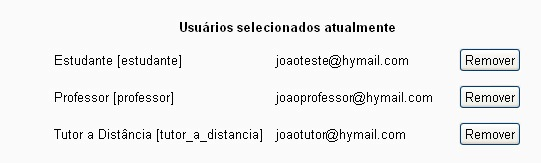
\includegraphics[width=0.7\textwidth]{imagem/cap3/fig9.jpg}}
  \caption{Configurar envio de Mensagens}
  \label{fig:confEnvio}
 \end{center}
\end{figure}

Clica-se em \textbf{Visualização} para ver o texto formatado e, por fim, envia-se a mensagem ou retorna-se para a edição do texto.


\section{Configuração da Disciplina}

Ao clicar no menu Configurações, disponível na página principal da disciplina, dispomos dos recursos descritos na Tabela \ref{tab:32}.


\begin{longtable}[htbp] {p{6cm}|p{9cm}}
  \hline
 \rowcolor[rgb]{0.8,0.8,0.8} \textbf{GERAL} &\\
 \hline
\textbf{Categoria Nome Completo} & Nome da disciplina por extenso. Na UFPB Virtual esse nome segue os padrões do SCA e não pode ser editado por professores ou tutores.\\
\hline

\textbf{Nome breve do curso} & Um nome curto da disciplina, onde se pode ver também o período. Igualmente não é editável, embora visível.\\\hline

\textbf{Número de identificação do curso} & Código da disciplina no SCA. Não pode ser alterado.\\\hline

\textbf{Sumário do curso} & Em um editor de texto pode ser colocada uma descrição breve da disciplina. Essa descrição aparecerá junto ao nome da disciplina na lista de cursos existente na página inicial do Moodle, conforme a figura abaixo:
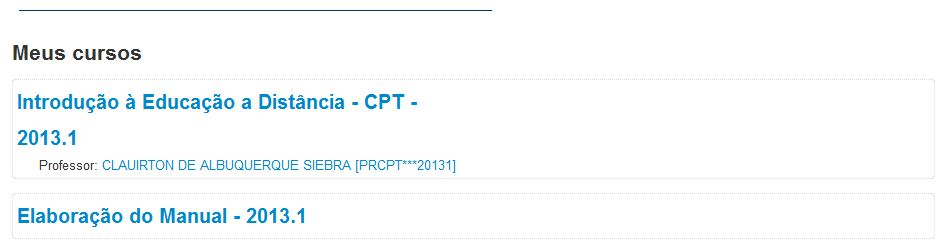
\includegraphics[width=0.6\textwidth]{imagem/cap3/fig25.jpg}\\\hline
\textbf{Formato} & \textbf{Formato Semanal: }
O professor estabelece a data de início e o número de semanas.\\
& \textbf{Formato Tópicos: }
Como no caso do curso semanal, o professor estabelece o número de tópicos e decide quais tópicos ocultar ou não.
Nos formatos Semanal e Tópicos, o Fórum de notícias é criado automaticamente.\\
& \textbf{Formato Social: }
Este formato é articulado em torno de um fórum principal que é publicado na página de abertura do curso. É um formato mais livre que pode ser usado, também, em contextos que não são cursos como, por exemplo, o quadro de avisos de um departamento.\\
& \textbf{Formato Scorm: }
Para se inserir conteúdo no padrão Scorm pode-se adicionar um recurso nesse padrão, ou criar uma disciplina em FORMATO SCORM. Essa opção é para usuários avançados, que tem conhecimento deste padrão e das ferramentas que o geram.
\\\hline
\textbf{Número de semanas ou tópicos} & Escolhe-se o número de semanas ou tópicos que a disciplina durará. Esse campo, aliado à data de início do curso, determinará as datas de cada semana, que o Moodle coloca automaticamente.\\\hline
\textbf{Data de início do curso} & Data do início do curso\\\hline
\textbf{Seções escondidas} & \textbf{Seções escondidas são mostradas contraídas:} significa que aquela semana ou tópico que for tornada oculta será mostrado ao estudante, porém com uma advertência: “não disponível”, não podendo ser acessada.\\
& \textbf{Seções escondidas são completamente invisíveis:} significa que o aluno não vê nada no lugar daquela semana ou tópico.
\\\hline
\textbf{Quantas notícias quer mostrar} & Esta configuração define o número de notícias recentes que serão visualizadas na página principal do curso, no bloco "Últimas Notícias".
Se você definir o valor como "0 itens" o bloco "Últimas Notícias" não será visualizado.
\\\hline
\textbf{Mostrar livro de notas aos estudantes} & Permite ou não a visualização do Quadro de Notas pelos alunos.\\\hline
\textbf{Mostrar relatório das atividades} & O relatório das atividades de cada usuário mostra todas as atividades daquele usuário no curso atual. Este relatório contém uma lista de todas as atividades realizadas e das mensagens individuais. Além disto, contém um arquivo detalhado de todos os acessos do usuário ao curso.
Os professores têm acesso constante a este relatório, que é disponível na página do perfil de cada usuário.
Escolhendo \textbf{SIM} ou \textbf{NÃO} é possível escolher a opção de mostrar, ou não, estes dados aos alunos.
\\\hline
\textbf{Tamanho máximo de upload} & O tamanho máximo de cada arquivo enviado para o site é definido para o Moodle inteiro pelo administrador da plataforma. Normalmente esse limite é definido também nas configurações do servidor.
Porém o professor pode, na sua disciplina, definir um valor menor do que o limite geral, escolhendo dentre os valores apresentados.\\\hline
%%%%%%%%%%%%%%%%%%%%%%%%%%%%%%%%%%%%%%%%%%%%%%%%%%%%%%%%%%%%%%%%%%%%%%%%%%%%%%%%%%%%%%%%%%%%%%%%%%%%%%%%%%%%%
\rowcolor[rgb]{0.8,0.8,0.8} \textbf{ACESSO COMO VISITANTE}&\\\hline
\textbf{Permitir o acesso de visitantes} & Visitantes são usuários não autenticados, ou que não fizeram login, aos quais é permitida uma visita à plataforma, sem permissão para participar ou alterar nada. Pode-se permitir, ou não, o acesso de visitantes a uma disciplina, sem que precisem estar matriculados na mesma.\\\hline
\textbf{Senha} & No caso de se permitir visitantes à disciplina, é possível criar uma senha para restringir o acesso a quem conheça a chave.\\\hline
\rowcolor[rgb]{0.8,0.8,0.8} \textbf{GRUPOS}&\\\hline
\textbf{Modalidade grupo} & Esta configuração possui três opções:\\
&\textbf{Nenhum grupo} - Não há subgrupos, todos fazem parte de uma grande comunidade;\\
&\textbf{Grupos separados} - Cada membro de grupo pode ver apenas seu próprio grupo, os outros são invisíveis;\\
&\textbf{Grupos visíveis} - Cada membro do grupo trabalha no seu próprio grupo, mas pode também ver outros grupos;
O tipo de grupo definido no nível da disciplina é o padrão para todas as atividades do curso. Cada atividade que suporta grupos pode também definir seu próprio tipo de grupo.
\\\hline
\textbf{Forçar modalidade grupo}& Se o modo de grupo é forçado, então o modo de grupo é aplicado a todas as atividades da disciplina. Configurações do modo de grupo de cada atividade serão ignoradas.\\\hline
\textbf{Agrupamento padrão} & Nas configurações de grupos da disciplina, clicando na aba Agrupamentos, é possível criar agrupamentos de grupos, que aparecerão nesta opção para escolha do agrupamento padrão. Se não houver agrupamentos somente haverá a opção Nenhum.\\\hline
%%%%%%%%%%%%%%%%%%%%%%%%%%%%%%%%%%%%%%%%%%%%%%%%%%%%%%%%%%%%%%%%%%%%%%%%%%%%%%%%%%%%%%%%%%%%%%%%%%%%%%%%%%%%%
\rowcolor[rgb]{0.8,0.8,0.8} \textbf{DISPONIBILIDADE}&\\\hline
\textbf{Disponibilidade }& A opção \textbf{Esse curso pode ser acessado pelos participantes} é o padrão. Escolhendo a opção \textbf{Esse curso não pode ser acessado pelos participantes}, a disciplina fica oculta.\\\hline

%%%%%%%%%%%%%%%%%%%%%%%%%%%%%%%%%%%%%%%%%%%%%%%%%%%%%%%%%%%%%%%%%%%%%%%%%%%%%%%%%%%%%%%%%%%%%%%%%%%%%%%%%%%%%
\rowcolor[rgb]{0.8,0.8,0.8} \textbf{IDIOMA}&\\\hline
\textbf{Forçar língua} & O padrão é \textbf{NÃO FORÇAR}. Pode-se optar por forçar alguns dos idiomas disponíveis, como por exemplo: Português - Brasil (pt\_br). Nesse caso a mudança de idioma na plataforma não surtirá efeito na disciplina.\\\hline

%%%%%%%%%%%%%%%%%%%%%%%%%%%%%%%%%%%%%%%%%%%%%%%%%%%%%%%%%%%%%%%%%%%%%%%%%%%%%%%%%%%%%%%%%%%%%%%%%%%%%%%%%%%%%
\rowcolor[rgb]{0.8,0.8,0.8} \textbf{RENOMEAR PAPEL (FUNÇÃO)}&\\\hline
 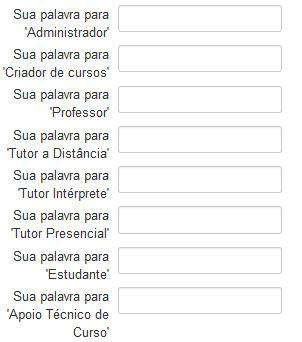
\includegraphics[width=4cm]{imagem/cap3/fig10.jpg} & As principais funções presentes na disciplina podem ser renomeadas. Isso fará com que sejam apresentadas com o novo nome em determinados locais dentro da disciplina, como quando se filtra os Participantes por sua função (papel atual), etc.
Ao clicar-se em Mostrar Avançado, ao lado deste quadro, algumas outras funções serão acrescentadas a lista para renomear.\\\hline
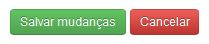
\includegraphics[width=3cm]{imagem/cap3/fig11.jpg} & Ao terminar de configurar a disciplina deve-se SALVAR.\\\hline
\caption{Itens de Configuração da Disciplina}
\label{tab:32}
\end{longtable}

\section{Configurações/Filtros}
Ao selecionar o item \textbf{Filtros no bloco Configurações}, dentro de uma disciplina, pode-se habilitar ou desabilitar os filtros presentes na plataforma (Veja a Figura \ref{Fig: filtroConf}).
\begin{figure}[htbp]
 \begin{center}
 \fbox{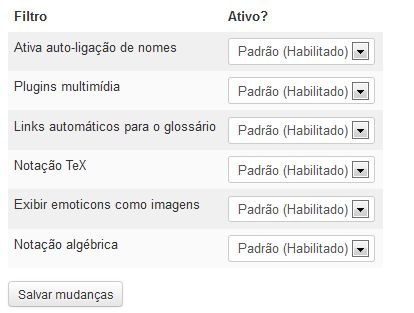
\includegraphics[width=0.4\textwidth]{imagem/cap3/fig12.jpg}}
  \caption{Filtro do bloco de Configurações}
  \label{Fig: filtroConf}
 \end{center}
\end{figure}
As mudanças feitas aqui serão válidas somente dentro da disciplina.

\section{Configurações/BackUp}
Ao clicar-se em \textbf{Backup} tem início uma sequência de páginas com os passos de configuração para se obter uma cópia da disciplina para uma futura restauração (Veja Figura \ref{Fig: confBackup}).

\begin{figure}[htbp]
 \begin{center}
 \fbox{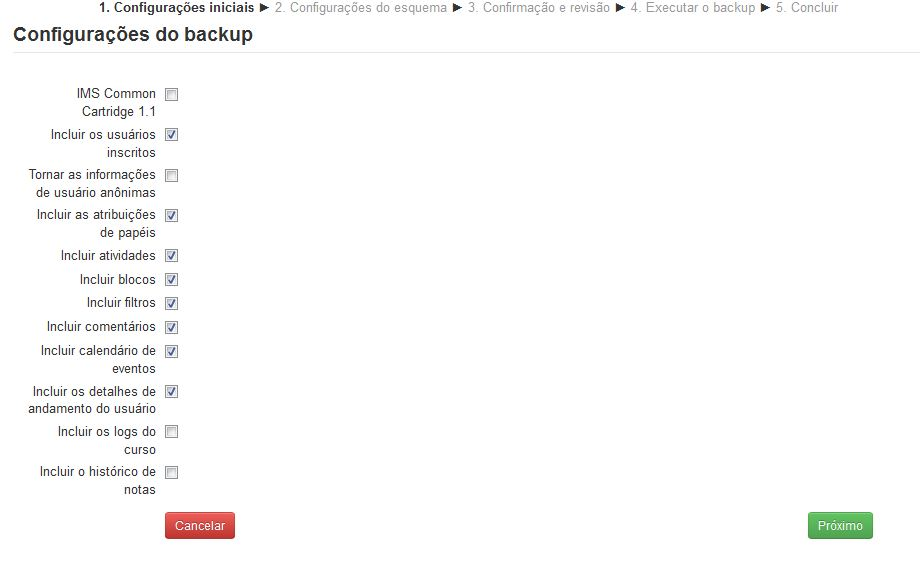
\includegraphics[width=0.8\textwidth]{imagem/cap3/fig13.jpg}}
  \caption{Configuração do Backup}
  \label{Fig: confBackup}
 \end{center}
\end{figure}

Na primeira tela escolhem-se os itens que irão fazer parte do backup. Dependendo das permissões de cada usuário alguns desses itens não farão parte da cópia obtida, ou não permitirão opção de escolha. Na Figura~\ref{Fig: confBackup}, na configuração padrão do Moodle para professores, somente os itens “Incluir Atividades”, “Incluir blocos” e “Incluir filtros” permitem escolha. Ao término, clica-se em \textbf{Próximo}.

A segunda tela, illustrada na Figura \ref{Fig: sentAtiv}), nos traz as \textbf{Semanas e as Atividades}, uma a uma, com a opção de selecionar ou não, para o caso de querermos um backup de somente alguns tipos de atividades, por exemplo, ou de somente uma semana, ou tópico. E assim por diante. Ao final, clica-se em \textbf{Próximo}.

\begin{figure}[htbp]
 \begin{center}
 \fbox{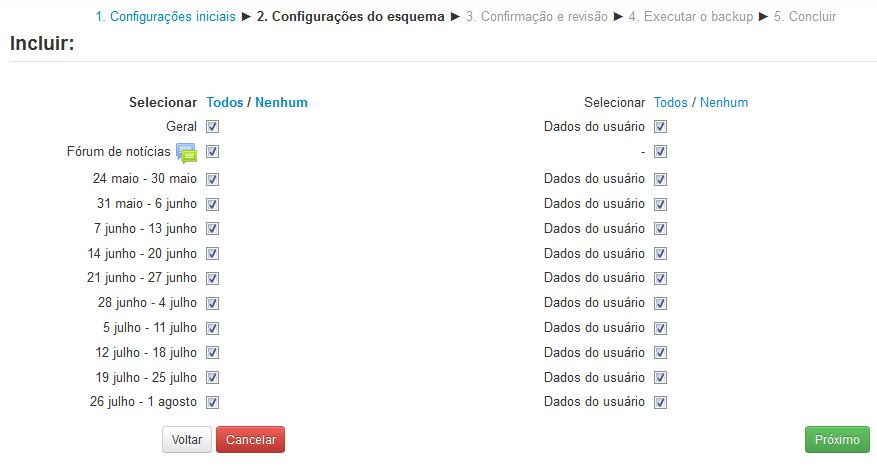
\includegraphics[width=0.6\textwidth]{imagem/cap3/fig14.jpg}}
  \caption{Semanas e atividades}
  \label{Fig: sentAtiv}
 \end{center}
\end{figure}

Após esse passo é mostrada uma lista das opções feitas para verificação. É também possível nomear o arquivo ZIP que será gerado (Veja a Figura \ref{Fig: envioBackup}).

\begin{figure}[htbp]
 \begin{center}
 \fbox{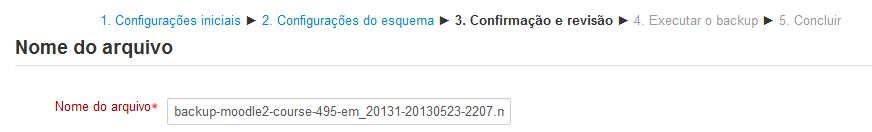
\includegraphics[width=0.6\textwidth]{imagem/cap3/fig15.jpg}}
  \caption{Envio de Backup}
  \label{Fig: envioBackup}
 \end{center}
\end{figure}

Tendo conferido todas as opções selecionadas e dados inserigos, clica-se em \textbf{Executar o Backup} para iniciar o processo de cópia. É necessário esperar alguns instantes, dependendo da quantidade de conteúdos da disciplina e das escolhas feitas previamente. Ao finalizar o processamento do backup aparecerá uma mensagem parecida a aquela na Figura \ref{Fig: confEnvio}.

\begin{figure}[htbp]
 \begin{center}
 \fbox{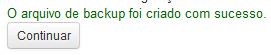
\includegraphics[width=0.6\textwidth]{imagem/cap3/fig16.jpg}}
  \caption{Confirmação de Envio}
  \label{Fig: confEnvio}
 \end{center}
\end{figure}
Clicando-se em \textbf{Continuar abre uma listagem de Backups} (Veja a Figura \ref{Fig: genrecBackup}), onde se pode restaurar o arquivo gerado (\textcolor{blue}{Restaurar}), baixar para o computador do usuário (\textcolor{blue}{Download}), ao lado de cada arquivo da lista e gerenciar os arquivos existentes, e clicando no botão \textbf{Gerenciar os arquivos de backup}, outras funcionalidade podem ser usadas.
\begin{figure}[htbp]
 \begin{center}
 \fbox{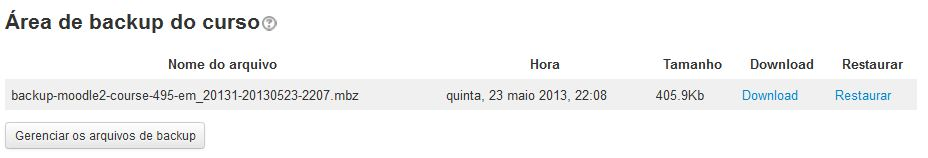
\includegraphics[width=0.7\textwidth]{imagem/cap3/fig17.jpg}}
  \caption{Gerenciar Backups}
  \label{Fig: genrecBackup}
 \end{center}
\end{figure}

Essas funcionalidades extras ao gerenciar os arquivos de backup, podem ser vistas na Figura \ref{Fig: genrecExtraBackup}. Pode-se acrescentar arquivos, tanto originados de outro diretório no servidor, quanto do computador do usuário, pode-se baixar os arquivos existentes em lote (todos), e ao clicar ao lado do nome do arquivo aparece um menu de contexto ligado a este, que permite baixá-lo, mudar o nome, mover e excluir (se o formato for .zip aparece também a funcionalidade \textbf{Descompactar}).

\begin{figure}[htbp]
 \begin{center}
 \fbox{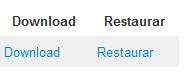
\includegraphics[width=0.3\textwidth]{imagem/cap3/fig18.jpg}}
  \caption{Funcionalidades Extras na Gerencia dos Backups}
  \label{Fig: genrecExtraBackup}
 \end{center}
\end{figure}

\section{Configurações/Restaurar}
\label{chap3:sec:restaurar}
Ao se escolher \textbf{Restaurar}, no bloco \textbf{Configurações} de uma disciplina, abrirá a mesma página que aparece ao fim do backup (Veja a Figura \ref{Fig: genrecBackup}).
As mesmas informações descritas acima também cabem aqui integralmente.
Ao clicar em \textcolor{blue}{Restaurar} uma sequência de sete passos é iniciada. A cada um é possível voltar ao anterior, ou avançar.

\begin{enumerate}
 \item \textbf{Confirmar:} informações sobre o backup, com a versão do moodle, formato, etc.; sobre a configuração do backup realizado quando da criação do arquivo; os detalhes do curso, suas seções e atividades, são listadas. Todas as informações são somente para conferência, não permitindo mudanças.
 
 \item \textbf{Destino:} nesta etapa decide-se se:
esse conteúdo será acrescentado ao já existente, ou
se o conteúdo do arquivo de backup sobreporá o conteúdo existente na disciplina.

\item \textbf{Configurações:} algumas configurações do backup são agora apresentadas na restauração, permitindo que se mantenha, ou se retire certos itens.

\item \textbf{Esquema:} uma lista de todas as seções (semanas ou tópicos) e atividades disciplinares presentes no backup. É possível desmarcar uma ou mais seções e atividades, caso seja do interesse restaurar somente algumas e não outras. É possível também renomear a disciplina, assim como escolher se as seções do backup sobreporão as já existentes na disciplina.

\item \textbf{Revisar:} todas as configurações e conteúdo escolhido são listados novamente, para conferência. Caso tudo esteja dentro do esperado, clica-se no botão \textbf{Executar a Restauração} para iniciar o \textbf{Processamento} do pedido de restauração. 
Após um breve período de tempo, dependendo do tamanho do backup, o processo concluí com uma mensagem parecida com aquela na 
Figura \ref{Fig: fim}.
\end{enumerate}

Ao clicar no botão Continuar abre novamente a página da disciplina, já restaurada.


\begin{figure}[htbp]
 \begin{center}
 \fbox{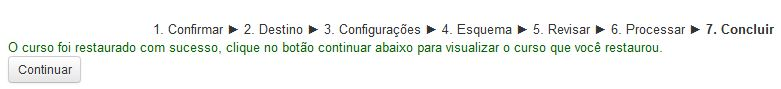
\includegraphics[width=0.8\textwidth]{imagem/cap3/fig19.jpg}}
  \caption{Conclusão do Processo de Configuração/Restauração}
  \label{Fig: fim}
 \end{center}
\end{figure}


\section{Configurações/Importar}
Essa é uma funcionalidade semelhante à restauração de backup. Porém ao invés de se usar um arquivo, pode-se importar diretamente de outra disciplina existente na mesma plataforma.

Cabe aqui explicar que o nível de permissão do usuário afetará diretamente a importação. Um professor, por exemplo,  poderá somente importar as suas próprias disciplinas, ou melhor, as disciplinas onde seja titular. É uma função útil pois permite importar o conteúdo de uma disciplina dada em um período anterior (Veja a Figura \ref{Fig: cap3_20}).

\begin{figure}[htbp]
 \begin{center}
 \fbox{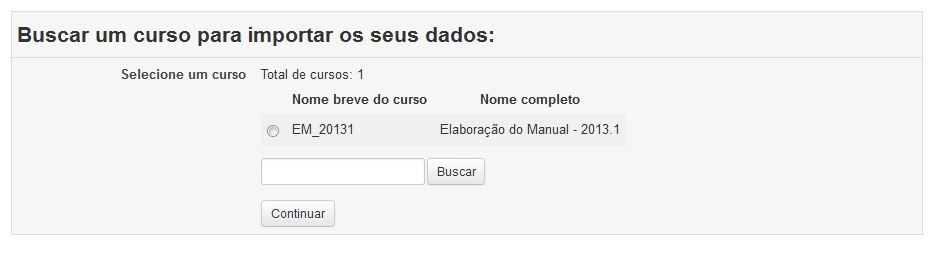
\includegraphics[width=0.7\textwidth]{imagem/cap3/fig20.jpg}}
  \caption{Importação de Dados}
  \label{Fig: cap3_20}
 \end{center}
\end{figure}

Ao escolher uma disciplina a ser importada, clica-se em \textbf{Continuar}. Novamente teremos a execução das etapas descritas na Seção~\ref{chap3:sec:restaurar} (Veja a Figura \ref{Fig: cap3_21}).
Em \textbf{Configurações iniciais} pode-se retirar ou manter algumas configurações da disciplina a ser importada, conforme a imagem 
na Figura \ref{Fig: cap3_21}.

\begin{figure}[htbp]
 \begin{center}
 \fbox{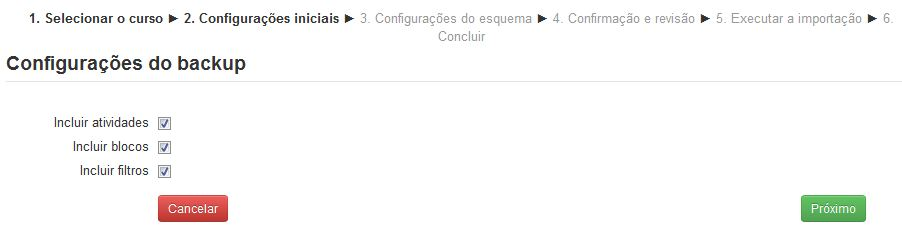
\includegraphics[width=0.8\textwidth]{imagem/cap3/fig21.jpg}}
  \caption{Importação de Disciplina}
  \label{Fig: cap3_21}
 \end{center}
\end{figure}



O terceiro passo, \textbf{Configurações do esquema} (Fig. \ref{Fig: cap3_22}), permite a escolha de certas semanas (ou tópicos) e das atividades e recursos que se quer importar.

\begin{figure}[htbp]
 \begin{center}
 \fbox{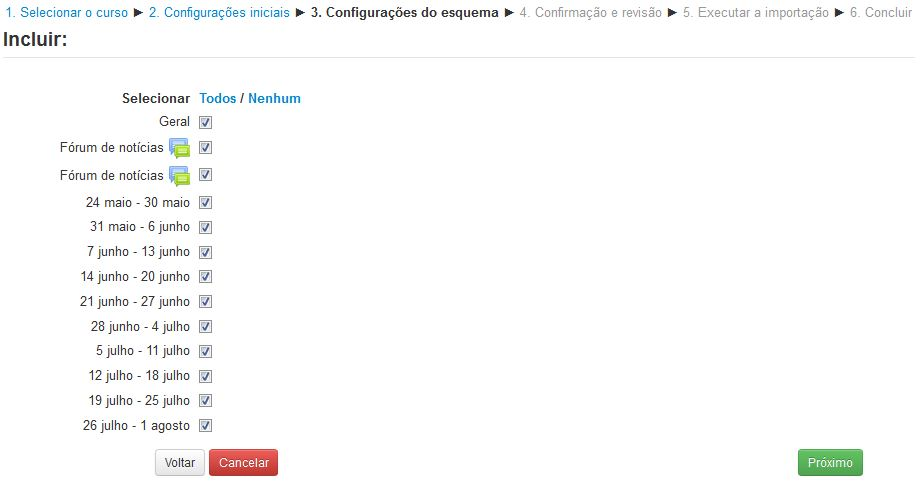
\includegraphics[width=0.7\textwidth]{imagem/cap3/fig22.jpg}}
  \caption{Configuração de Esquema}
  \label{Fig: cap3_22}
 \end{center}
\end{figure}

A quarta etapa, \textbf{Confirmação e revisão}, listará as escolhas feitas. Lembrando que sempre é possível voltar às etapas anteriores. Após conferir os dados inseridos, clica-se no botão \textbf{Executar a importação}.

Ao final de alguns instantes, enquanto o sistema executa a importação, chega-se a etapa final, \textbf{Concluir}, com a apresentação da mensagem 
na Figura~\ref{Fig: cap3_23}.

\begin{figure}[htbp]
 \begin{center}
 \fbox{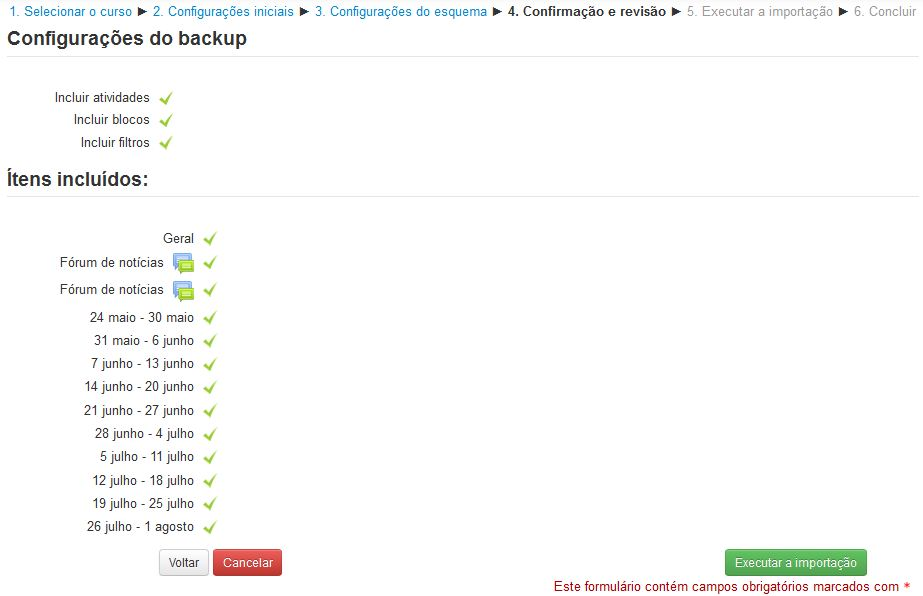
\includegraphics[width=0.6\textwidth]{imagem/cap3/fig23.jpg}}
  \caption{Configuração de Esquema}
  \label{Fig: cap3_23}
 \end{center}
\end{figure}

\section{Configurações/Reconfigurar (course/reset)}
Esta página permite que você esvazie os dados de uma disciplina, sem excluir as atividades e outras configurações (Conforme a Tabela \ref{tab:Conf3}), no caso de eventual reaproveitamento para outro período. As exclusões não poderão ser revertidas.

\begin{longtable}[htbp!]{p{6cm}|p{9cm}}
\hline
%%%%%%%%%%%%%%%%%%%%%%%%%%%%%%%%%%%%%%%%%%%%%%%%%%%%%%%%%%%%%%%%%%%%%%%%%%%%%%%%%%%%%%%%%%%%%%%%%%%%%%%%%%%%%
\rowcolor[rgb]{0.8,0.8,0.8} \textbf{GERAL}&\\\hline
\textbf{Data de início do curso} & Esta configuração determina o início da primeira semana para um curso em formato semanal. Também determina a data inicial em que os logs das atividades do curso estarão disponíveis. No caso de atividades herdadas da antiga disciplina, ou já existentes, o Moodle reconfigura a data de início e fim da atividade, em função da semana onde está inserida.\\\hline
\textbf{Excluir eventos} & Seleciona-se caso queira excluir todos os eventos da disciplina\\\hline
\textbf{Excluir logs} & Seleciona-se para excluir todos os logs da disciplina.\\\hline
\textbf{Excluir todas as anotações} & Seleciona-se para excluir todas as anotações na disciplina.\\\hline
\textbf{Excluir todos os comentários} & Seleciona-se para excluir todos os comentários (feedbacks) da disciplina.\\\hline
\textbf{Excluir dados de conclusão de curso} & Seleciona-se para excluir todos os dados de conclusão de curso da disciplina.\\\hline
\textbf{Apagar de associações de blog} & Se selecionado, as mensagens do blog não serão mais associadas a esta disciplina ou a atividades ou recursos da disciplina. As mensagens não serão apagadas.\\\hline
%%%%%%%%%%%%%%%%%%%%%%%%%%%%%%%%%%%%%%%%%%%%%%%%%%%%%%%%%%%%%%%%%%%%%%%%%%%%%%%%%%%%%%%%%%%%%%%%%%%%%%%%%%%%%
\rowcolor[rgb]{0.8,0.8,0.8} \textbf{FUNÇÕES}&\\\hline
\textbf{Cancelar inscrições} & Marcam-se as funções que se quer cancelar, como tutores, ou estudantes. Pode-se pressionar a tecla Ctrl para selecionar mais de uma função.\\\hline
\textbf{Excluir todas as sobreposições no curso \textcolor{blue}{$\ast$}} & Ao marcar-se essa opção todas as permissões de usuário que tenham sido modificadas somente dentro da disciplina, voltarão ao padrão da plataforma.\\\hline
\textbf{Excluir todas as designações de funções locais} & O mesmo que Cancelar inscrições, porém equivale a marcar todas as funções existentes.\\\hline
%%%%%%%%%%%%%%%%%%%%%%%%%%%%%%%%%%%%%%%%%%%%%%%%%%%%%%%%%%%%%%%%%%%%%%%%%%%%%%%%%%%%%%%%%%%%%%%%%%%%%%%%%%%%%
\rowcolor[rgb]{0.8,0.8,0.8} \textbf{LIVRO DE NOTAS}&\\\hline
\textbf{Remova todos os itens e categorias} & Seleciona-se para excluir, no Quadro de Notas da disciplina, todos os itens de nota e categorias que tenham sido criados até então.\\\hline
\textbf{Remova todas as notas} & Ao selecionar-se essa opção todas as notas na disciplina serão excluídas.\\\hline
%%%%%%%%%%%%%%%%%%%%%%%%%%%%%%%%%%%%%%%%%%%%%%%%%%%%%%%%%%%%%%%%%%%%%%%%%%%%%%%%%%%%%%%%%%%%%%%%%%%%%%%%%%%%%
\rowcolor[rgb]{0.8,0.8,0.8} \textbf{GRUPOS}&\\\hline
\textbf{Excluir todos os grupos \textcolor{blue}{$\ast$}} & Exclui todos os grupos criados na disciplina. Note que os pólos são grupos e, eventualmente, não devem ser apagados.\\\hline
\textbf{Remover todos os membros do grupo \textcolor{blue}{$\ast$}} & Retira os membros de cada grupo, mantendo os grupos.\\\hline
\textbf{Excluir todos os agrupamentos \textcolor{blue}{$\ast$}} & Os agrupamentos são grupos de grupos. Essa opção, se marcada, reconfigurará a disciplina sem os agrupamentos existentes.\\\hline
\textbf{Remover todos os grupos dos agrupamentos \textcolor{blue}{$\ast$}} & Ao marcar-se essa opção todos os grupos do agrupamento serão removidos.\\\hline
%%%%%%%%%%%%%%%%%%%%%%%%%%%%%%%%%%%%%%%%%%%%%%%%%%%%%%%%%%%%%%%%%%%%%%%%%%%%%%%%%%%%%%%%%%%%%%%%%%%%%%%%%%%%%
\rowcolor[rgb]{0.8,0.8,0.8} \textbf{TAREFAS}&\\\hline
\textbf{Excluir todos os arquivos enviados} & Exclui os arquivos enviados nas atividades existentes da disciplina.\\\hline
%%%%%%%%%%%%%%%%%%%%%%%%%%%%%%%%%%%%%%%%%%%%%%%%%%%%%%%%%%%%%%%%%%%%%%%%%%%%%%%%%%%%%%%%%%%%%%%%%%%%%%%%%%%%%
\rowcolor[rgb]{0.8,0.8,0.8} \textbf{CHATS}&\\\hline
\textbf{Remover todas as mensagens} & Exclui todas as mensagens dos bate-papos (chats) existentes na disciplina.\\\hline
%%%%%%%%%%%%%%%%%%%%%%%%%%%%%%%%%%%%%%%%%%%%%%%%%%%%%%%%%%%%%%%%%%%%%%%%%%%%%%%%%%%%%%%%%%%%%%%%%%%%%%%%%%%%%
\rowcolor[rgb]{0.8,0.8,0.8} \textbf{FÓRUNS}&\\\hline
\textbf{Excluir todas as mensagens} & Exclui todas as mensagens de todos os fóruns da disciplina.\\\hline
\textbf{Excluir as mensagens de \textcolor{blue}{$\ast$}} & Exclui as mensagens dos fóruns filtrados por tipo de fórum.
Ex: fórum geral, fórum de notícias, etc.\\\hline
\textbf{Excluir todas as subscrições \textcolor{blue}{$\ast$}} & Aqui subscrição é usada para quando um usuário se torna assinante de um fórum. Ao se tornar assinante, ele passa a receber as mensagens desse fórum por e-mail. Selecionando esse item essas subscrições são excluídas.\\\hline
\textbf{Excluir todas as preferências de rastreamento dos fóruns \textcolor{blue}{$\ast$}} & Ao subscrever um fórum o usuário pode escolher se receberá por email, ou outras preferências. Ao se marcar esse item essas preferências serão excluídas. \\\hline
\textbf{Excluir todas as pontuações} & Exclui todos os pontos dados às participações nos fóruns desta disciplina.\\\hline
\caption{Descrição das opções de configuração e re-configuração de disciplinas.}
  \label{tab:Conf3}
\end{longtable}
(\textcolor{blue}{$\ast$})Esta é uma opção avançada e pode ser acessada somente se o botão \textbf{Mostrar Avançado} for clicado.

Na parte de baixo da página de reconfiguração há quatro botões, os quais dois são descritos na Figura \ref{fig:cap3_24}, enquanto 
que os botões \textbf{Desmarcar todas as seleções} e \textbf{Cancelar} são auto-explicativos.

\begin{figure}[htbp]
 \begin{center}
 \fbox{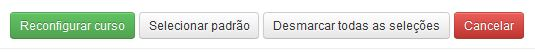
\includegraphics[width=0.5\textwidth]{imagem/cap3/fig24.jpg}}
  \caption{Configurações da Disciplina}
  \label{fig:cap3_24}
 \end{center}
\end{figure}
